\documentclass[french]{article}
\usepackage[utf8x]{inputenc}
\usepackage[T1]{fontenc}
\usepackage{babel}
\usepackage{lmodern}
\usepackage[top=2cm,bottom=2cm,left=3cm,right=3cm]{geometry}
\usepackage{microtype}
\usepackage{mathtools, amssymb, amsthm}
\usepackage{mdframed}
\usepackage{hyperref}
\usepackage{graphicx}
\usepackage{xcolor}
\usepackage{mathrsfs}
\usepackage{wrapfig}
\usepackage{stmaryrd}
\usepackage{dsfont}
\usepackage{framed}
\usepackage{marginnote}
\usepackage[Glenn]{fncychap}

\theoremstyle{definition}
\newtheorem{prototheorem}{Théorème}[section]
\newenvironment{thm}
   {\colorlet{shadecolor}{orange!10}\begin{shaded}\begin{prototheorem}}
   {\end{prototheorem}\end{shaded}}

\newtheorem*{protocorollary}{Corollaire}
\newenvironment{corollary}
    {\colorlet{shadecolor}{violet!10}\begin{shaded}\begin{protocorollary}}
    {\end{protocorollary}\end{shaded}}

\newtheorem*{protolemma}{Lemme}
\newenvironment{lemma}
    {\colorlet{shadecolor}{pink!15}\begin{shaded}\begin{protolemma}}
    {\end{protolemma}\end{shaded}}


\newtheorem{protodefinition}{Définition}[section]
\newenvironment{definition}
    {\colorlet{shadecolor}{green!5}\begin{shaded}\begin{protodefinition}}
    {\end{protodefinition}\end{shaded}}

\newtheorem{protoproposition}{Proposition}[section]
\newenvironment{prop}
    {\colorlet{shadecolor}{blue!5}\begin{shaded}\begin{protoproposition}}
    {\end{protoproposition}\end{shaded}}

\newtheorem{protoremark}{Remarque}[section]
\newenvironment{remark}
    {\colorlet{shadecolor}{yellow!5}\begin{shaded}\begin{protoremark}}
    {\end{protoremark}\end{shaded}}

\newtheorem{exo}{Exercice}
\newtheorem*{protoexemple}{Exemple}
\newenvironment{exemple}
    {\colorlet{shadecolor}{gray!10}\begin{shaded}\begin{protoexemple}}
    {\end{protoexemple}\end{shaded}}


%\newcommand{\lesss}{\rotatebox[origin=c]{90}{$\land$}}
%\newcommand{\less}{\ \lesss\ }

%\newcommand{\biggg}{\rotatebox[origin=c]{90}{$\lor$}}
%\newcommand{\bg}{\ \biggg\ }

\newcommand{\R}{\mathbb{R}}

\newcommand{\less}{<}

\newcommand{\bg}{>}


\title{\bsc{Approximation des EDP}}
\author{Mohammad Reza \bsc{Pakzad}}
\date{2023-2024}

\begin{document}

\maketitle

\tableofcontents

\newpage

\marginnote{17-01-2024}

\textbf{EDP} : abbreviation pour ``équations aux dérivées partielles''. De là, deux grandes théories émergent : analyse des EDP (aspect théorique) et méthode pour la résolution numérique. Entre les deux, il y a la théorie de l'approximation des EDP.

%fig-approx-courbes

Il n'y a pas de théorie unique qui s'applique à toutes les EDP.

Dans ce cours, on abordera surtout les équations de type \(\Delta u = f\).

\section*{Quelques notations}
\addcontentsline{toc}{section}{Quelques notations}

\(\Omega \subseteq \mathbb{R}^n\) ouvert.

\(u : \Omega \longrightarrow \mathbb{R}^m\), avec

\[u(x_1, \dots, x_n) = (u ^{1}(x_1, \dots,x_n), u ^{m}(x_1, \dots, x_n)).\]

Pour tout \(i\), \(u _{x_i}(x) = \displaystyle\frac{\partial u }{\partial x_i}(x) = \lim_{h \to 0} \frac{u(x+ h e_i) - u(x)}{h} = \partial _{x_i}u(x) = \partial_i u(x)\) (on utilise la dernière notation quand il n'y a pas d'ambiguité).

Notez que

\[u _{x_i} = (u _{x_i}^{1}, \dots, u _{x_i}^{m}).\]

Aussi \(u _{x_i x_j} = \displaystyle\frac{\partial  }{\partial x_j}(u x_i) = \displaystyle\frac{\partial  }{\partial x_j}\left(\displaystyle\frac{\partial u }{\partial x_i} \right)  = \displaystyle\frac{\partial ^2 u }{\partial x_j x_i}\), de même pour les dérivées de tout ordre.

\begin{exemple}
  Pour \(m =1, n=1, u(t,x) = (e^{-t}x, x ^2 + t)\).

  On a

  \[u_t = (- e^{-t}x, 1), u_x = (e^{-t}, 2x).\]

\end{exemple}

\subsection*{Le gradient et la jacobienne}
\addcontentsline{toc}{subsection}{Le gradient et la jacobienne}

Si \(m=1, u : \Omega \longrightarrow \mathbb{R}, \nabla u = D u \operatorname{grad}u = [\partial _{x_1}, \dots, \partial _{x_n}u] : \Omega \longrightarrow \mathbb{R}^n\).

Si \(m \bg 1\), on a affaire à une matrice jacobienne de taille \(m \times n\). Le gradient est un cas particulier de la jacobienne.

\[\nabla u = \begin{bmatrix}
  \displaystyle\frac{\partial u ^{1} }{\partial x_1} & \dots & \displaystyle\frac{\partial u ^{1} }{\partial x_n}\\
  \vdots & \ddots & \vdots \\
  \displaystyle\frac{\partial u ^{m} }{\partial x_1}  & \dots & \displaystyle\frac{\partial u ^{m} }{\partial x_n}
\end{bmatrix}.\]

\subsection*{La divergence}
\addcontentsline{toc}{subsection}{La divergence}

Si \(\overrightarrow{F} : \Omega \longrightarrow \mathbb{R}^n\) est une application linéaire, avec \(\overrightarrow{F}(x) = (F ^{1}(x), \dots, F ^{n}(x))\), on a

\[\operatorname{div} \overrightarrow{F} = \partial _{x_1} F ^{1}+ \dots + \partial _{x_n}F ^{n} = \displaystyle\sum_{i=1}^{n}F _{x_i}^{i} : \Omega \longrightarrow \mathbb{R}.\]

On peut aussi dire que \(\operatorname{div}\overrightarrow{F} = \nabla \cdot \overrightarrow{F}\).

\begin{remark} \marginnote{{\fontencoding{U}\fontfamily{futs}\selectfont\char 66\relax}}
  Si \(\overrightarrow{F} = (0,T) \times \Omega \longrightarrow \mathbb{R}^n\) (c'est-à-dire \(\overrightarrow{F}\) dépend aussi du temps),

  \[\operatorname{div}\overrightarrow{F} = \operatorname{div}_t \overrightarrow{F}(t,x) = F _{x_1}^{1}+ \dots + F _{x_n}^{n}(t,x).\]
\end{remark}

\subsection*{Le laplacien}
\addcontentsline{toc}{subsection}{Examen de l'année dernière}

On définit

\[\Delta u := \partial _{x_1 x_1} + \dots \partial _{x_n x_n} = \operatorname{div}(\nabla u) = \nabla \cdot(\nabla u)\]

et si \(u =(u ^{1}, \dots u ^{m})\), alors

\[\Delta u := (\Delta u ^{1}, \dots, \Delta ^{m}).\]

Encore \(\Delta u : div (D u)\) où \(A := \Omega \longrightarrow \mathbb{R} ^{m \times n}\), où \(A = [\overrightarrow{v}^{1}, \dots, \overrightarrow{v}^{n}]\), avec \(\overrightarrow{v}^{j} : \Omega \longrightarrow \mathbb{R}^m\), on définit

\[div A : \partial _{x_1} \overrightarrow{v}^{1} + \dots + \partial _{x_n}\overrightarrow{v}^{n}.\]

Ici on a identifié \(\Delta u = (\Delta u ^{1}, \dots, \Delta ^{m})\) comme un vecteur ligne avec le vecteur colonne qui est

\[div (Du) = \begin{bmatrix}
  div \nabla u ^{1}\\
  \vdots \\
  div \nabla u ^{1}
\end{bmatrix} = \begin{bmatrix}
  \Delta u ^{1}\\
  \vdots \\
  \Delta u ^{1}
\end{bmatrix}.\]

\section{Quelques exemples des EDP}

On cherche une ou plusieurs applications \(u : ? \longrightarrow ?\) satisfaisant

\subsection{L'équation de la chaleur en 1D (une dimension spatiale)}


\[ u : ]0,T[ \times [a,b] \longrightarrow \mathbb{R}, t \in ]0,T[, x \in [a,b],a,b,t \in \mathbb{R}, T \bg 0.\]

\(f : ]0,T[\times [a,b] \longrightarrow \mathbb{R}\) est donnée (la source), les données sont \(u_0(x), g_a(t), g_b(t)\), \(\alpha \in \mathbb{R}\). L'équation est la suivante :

\begin{equation}\label{chaleur}
  \begin{cases}
    u_t - \alpha ^2 u _{xx} = f \text{ (EDP)}  \\
    u(0,x) = u_0(x) \text{ (condition initiale, CI), } \forall x \in [a,b] \\
    \begin{cases}
      u(t,a) = g_a(t) \\
      u(t,b) = g_b(t), \forall t \in ]0,T[.
    \end{cases}
  \end{cases}
\end{equation}

Ce sont les valeurs limites aux bords (ou conditions aux bords) de type Dirichlet.

C'est un \textbf{problème d'évolution}.

%fig-chaleur

Cette équation s'appelle aussi l'équation de la diffusion.

%fig-diffus

Ici, l'équation de la chaleur a besoin de sa CI et de ses valeurs aux bords (VB) pour être bien posée (existence, unicité et stabilité d'une solution).

\(A = \alpha ^2\) est la conductivité (une constante).

Si la barre n'est pas homogène dans ses propriétés thermiques, on peut avoir une conductivité non constante.

\[A : [a,b] \longrightarrow \mathbb{R}^{+} := \{ y \in \mathbb{R} \mid y \bg 0 \}.\]

L'équation devient \(u_t - (A(x)u_x)_x = f\).

\subsection{L'équation de la chaleur en 2D, 3D ou \(n\)D}

L'équation de la chaleur (en deux, trois ou \(n\) dimensions). Soit \(\Omega \iota \mathbb{R}^n\) domaine spatial, \(\partial \Omega\) le bord de \(\Omega\) dans \(\mathbb{R}^n\).

Soit \(x \in \Omega, A(x) \in \mathbb{R}^{n \times n}_{\operatorname{sym}, \operatorname{pos}}\).

\begin{equation}\label{chaleur-nd}
  \begin{cases}
    u_t - div(A D u) = f \quad u,f : [0,T[ \times \Omega \longrightarrow \mathbb{R} \\
    u(0,x) = u_0(x) \text{ CI } \\
    u(t,x) = g(t,x) \quad (t,x) \in [0,T[ \times \partial \Omega \text{ VB }.
  \end{cases}
\end{equation}

Si \(A(x) = \alpha ^2 I\), l'équation devient \(u_t - \alpha ^2 \Delta u = f\).

\(u_t - div(A \nabla u)\) est l'équation parabolique de diffusion.

\subsection{L'équation des ondes en 1D}


L'équation des ondes (1D), aussi appelée l'équation d'Alembert.

\(u(t,x), t \in [0,T[, x \in [a,b]\). \(f(t,x)\) est donnée, \(\nu \in \mathbb{R}^+\), \(u_0(x), \nu_0(x), g_a(t), g_b(t)\).

\begin{equation}
  \begin{cases}
    \frac{1}{\nu ^2}u _{tt} - u _{xx} = f \\
    u(0,x) = u_0(x), u_t(0,x) = \nu_0(x) \text{ CI } \\
    u(t,a) = g_a(t), u(t,b) = g_b(t) \text{ VB.}
  \end{cases}
\end{equation}

%fig-corde

Si les deux bouts de la corde sont fixés, on peut imposer \(g_a(t) = g_b(t) = 0\).

L'équation des ondes est une équation \textbf{hyperbolique}.

\subsection{L'équation des ondes en 2D, 3D ou \(n\)D}

\(\Omega \in \mathbb{R}^n\).

\begin{equation}
  \begin{cases}
    \frac{1}{x ^2}u _{tt} - \Delta u = f \\
    u(0,x) = u_0(x), u_t(0,x), \nu_0(x) \text{ CI } \\
    u(t,x) = g(t,x), (t,x) \in [0,T[ \times \partial \Omega.
  \end{cases}
\end{equation}

\subsection{L'équation de Poisson}


\(\Omega \in \mathbb{R}^n, u(x), f(x), g(x), x \in \partial \Omega\).

\begin{equation}
  \begin{cases}
    - \Delta u = f \\
    u(x) = g(x), \forall x \in \partial \Omega \text{ VB de type Dirichlet.}
  \end{cases}
\end{equation}

C'est un problème aux limites de type elliptique.

\begin{remark}
  Si \(n=1\),

  \[\begin{cases}
    -u _{xx} = f \\
    u(a) = g_a, u(b) =g_b
  \end{cases}\]

  n'est pas une EDP, mais une EDO.
\end{remark}

%fig-neumann

\subsection{Généralisation de l'équation de Poisson}

C'est une équation scalaire elliptique d'ordre 2.

Soit \(A : \Omega \longrightarrow \mathbb{R}^{n \times n}\) symétrique positive, \(f : \Omega \longrightarrow \mathbb{R}, u : \Omega \longrightarrow \mathbb{R}\).

\begin{equation}\label{gen-poisson}
  \begin{cases}
    -div(A(x)\nabla u) = f \text{ dans } \Omega \\
    \text{ VB } \partial \Omega
  \end{cases}
\end{equation}

\begin{remark}
  Si \(\Omega \subseteq \mathbb{R}^n, a : \Omega \longrightarrow \mathbb{R}^{+}\) la conductivité, avec \(A(x) = a(x)\operatorname{id} _{n \times n}\), alors l'équation de la chaleur devient :

  \begin{equation*}
    u_t - div(a(x)\nabla u) = f \\
    \text{CI}\\
    \text{VB}.
  \end{equation*}

  Si \(u : \Omega \longrightarrow \mathbb{R}\) est la température en équlibre (\(u(t,x)\) ne change pas dans le temps), alors \(u_t(t,x) = 0\) implique que \(u(x):= u(t,x)\) est une solution de \ref{gen-poisson}.

  En général on s'attend à ce que si \(u _{\infty}\) satisfait \ref{gen-poisson} et \(u(t,x)\) est la solution de l'équation de la chaleur, alors

  \[\lim_{t \to \infty} u(t,x) = u _{\infty}(x).\]
\end{remark}

\subsection{L'équation de Navier-Stokes (2D/3D)}

Soit \(\Omega \subseteq \mathbb{R}^n, t \in [0,T[, x \in \Omega\), \(u(t,x) \in \mathbb{R}^n, u : [0,T[ \times \Omega \longrightarrow \mathbb{R}^n, p(t,x)\in \mathbb{R}^n\).

\(f : [0,T[ \times \Omega \longrightarrow \mathbb{R}^n\) donné, ainsi que \(u_0(x), g(t,x)\) donnés.

\(u_0 : \Omega \longrightarrow \mathbb{R}^n, g : [0,T[ \times \partial \Omega \longrightarrow \mathbb{R}^n\).


\begin{equation}\label{eqn:navier-stokes}
   \begin{cases}
     u_t + u \cdot \nabla u - \nu \Delta u + \Delta p = f \\
     div u = 0 \text{ (incompréssibilité ou continuité) } \\
     u(0,x) = u_0(x) \text{ CI} \\
     u(t,x) = g(t,x) \text{ VB de type Dirichlet (d'autre type sont possibles)}
   \end{cases}\tag{N.S.}
 \end{equation}


 \(u\) est la vitesse d'un fluide en un point \(x \in \Omega\).

 \(\nu\) est la [...] du fluide.

 \(p\) et la pression.

 Il faut résoudre \ref{eqn:navier-stokes} pour \(u\) et \(p\).

 \

 C'est une équation de mécanique des fluides.

 Notez le terme \(u \cdot \nabla u = [u \cdot \nabla u ^{1}, \dots, u \cdot \nabla u ^{n}]\), avec \(\nabla u = \nabla_x u = [\partial _{x_1}u, \dots, \partial _{x_n}u]\).

 \textbf{L'équation de l'équilibre de la quantité du mouvement fluide homogène de densité} \(f = \text{ constante.}\)

S'il y a une non-linéarité forte, alors il y a problème technique pour l'analyse.

\subsection{L'équation de transport}

\subsection{L'équation de Monge-Ampère (équation complément non-linéaire)}

\(u : \Omega \longrightarrow \mathbb{R}^2, Hu = \left[\displaystyle\frac{\partial ^2 u }{\partial x ^{i}x^{j}} \right] _{n \times n}\), \(f\) donné.

\begin{equation*}
  \operatorname{det}(Hu ) = f + VB.
\end{equation*}

\subsection{L'équation de la plaque élastique linéaire}

Soit \(\Omega \subseteq \mathbb{R}^n, u : \Omega \longrightarrow \mathbb{R}, f : \Omega \longrightarrow \mathbb{R}\) données, \(g : \partial \Omega \longrightarrow \mathbb{R}, h : \partial \Omega \mathbb{R}\).

\begin{equation}
  \Delta ^2 u = f \\
  u(x) = g(x) \\
  \displaystyle\frac{\partial u }{\partial \overrightarrow{n}}(x) = h(x), x \in \partial \Omega,
\end{equation}

avec \(\Delta ^2 u = \Delta(\Delta u) = \displaystyle\sum_{i=1}^{n}\partial _{ii}(\Delta u)\).

C'est l'équation de la plaque elastique linéaire \((n=2)\) avec le bord fixé.

\(u\) modélise le déplacement vertical de la plaque et \(f\) est la forme verticale.

\section{Méthode de différence finie (une méthode d'approximation des EDP)}

\subsection{Approximation des fonctions et leurs dérivées partielles}

\subsubsection{Théorème de Taylor}

\begin{thm}
  Soient \([a,b] \subseteq \mathbb{R}, u \in \mathcal{C} ^{n+1}([a,b]), c \in [a,b]\).

  Pour tout \(x \in [a,b]\), il existe \(z\) entre \(c\) et \(x\) tel que

  \[u(x) = T_n(x)+E _{n+1}(x),\]

  où \(T_n\) est le polynôme de degré \(\leq  n\), \(E _{n+1}\) est l'erreur (le reste) et

  \[T_n(x) = \displaystyle\sum_{k=0}^{n} \frac{u ^{(k)}}{k!}(x-c)^{k}, E _{n+1} = \frac{u ^{(n+1)}(z)}{(n+1)!}(x-c)^{n+1}.\]
\end{thm}

\begin{remark}
  \(T ^{(z)}(c) = u ^{(j)}(c), \forall 0 \leq j \leq n\).

  Si on remplace \(x\) par \((x+h)\) et \(c\) par \(x\), on obtient

  \[u(x+h) = \displaystyle\sum_{k=0}^{n} \frac{u ^{(k)}(x)}{k!} h ^{k} + \frac{u ^{(n+1)}(z)}{(n+1)!}h ^{n+1}.\]
\end{remark}

\subsubsection{La différence finie (D.F.)}

\begin{figure}[h!]
  \centering
  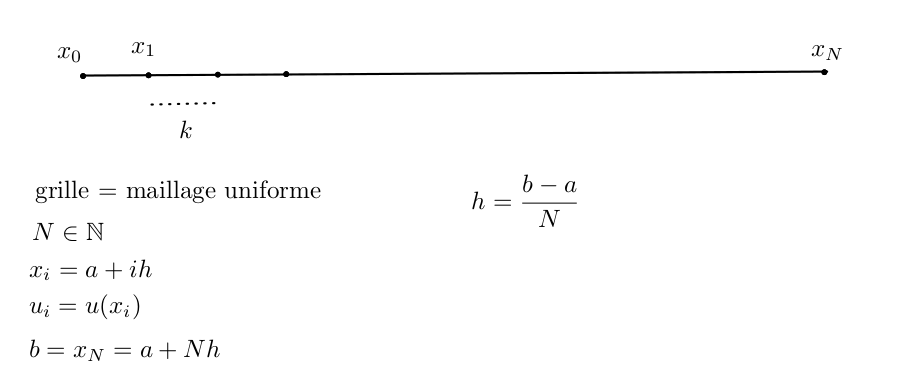
\includegraphics[scale=0.3]{figures/difference-finie.png}
  \caption{Méthode de la différence finie}
  \label{}
\end{figure}


\(u\) est approximé par les valeurs \(u_0, \dots, u_N\) (le \(u\) numérique). C'est ce que le logiciel va prendre en compte pour le représentant de l'application \(u\).

\begin{exemple}

  \

  \begin{enumerate}
    \item

    \begin{equation}\label{uiplus1}
      u _{i+1} = u(x _{i+1}) = u(x_i +h) = \frac{u(x_i)}{u_i} + u_x(x_i)h + \frac{u _{xx}}{2!}(x_i)h ^2 + \frac{u _{xxx}}{3!}(x_i)h ^3+ \dots
    \end{equation}

    \item

    \begin{equation}\label{uimoins1}
      u _{i-1} = u(x_i - h) = u(x_i) - u_x(x_i)h + u _{xx}(x_i)\frac{h ^2}{2} - u _{xxx}(x_i) \frac{h ^3}{3!}+ \dots
    \end{equation}
  \end{enumerate}
\end{exemple}

On a

\[\ref{uiplus1} \implies u_x(x_i) = \frac{u _{i+1} - u_i}{h} - \underbrace{\frac{1}{h} \left[\frac{u _{xx}(x_i)}{2}h ^2 + \frac{u _{xxx}(x_i)}{3!}h ^3+ \dots \right]}_{\text{ordre de grandeur de }h}.\]


\begin{exo}
  Si \(u \in \mathcal{C}^{n+1}([a,b])\), alors il existe \(c \bg 0\) tel que

  \[\left\lvert \frac{1}{h} \left[\displaystyle\sum_{k=2}^{n} \frac{u ^{(k)}(x_i)}{k!}h ^{k}+ \frac{u ^{n+1}}{(n+1)!}h ^{n+1}\right] \right\rvert \leq  Ch.\]
\end{exo}

Si une expression est uniformément majorée par \(Ch\) en sa valeur absolue, on dit qu'elle est \(O(h)\). Donc on a

\[u_n(x_i)= \underbrace{\frac{u _{i+1}- u_i}{h}}_{D ^{+}_x u_i} + O(h),\]

où \(D_x ^{+}u_i\) est la différence finie du premier ordre en avant de \(u_i\).


\[\ref{uimoins1} \implies u(x _{i-1}) = u(x_i),\]

\[u_x(x_i) = \frac{u_i - u _{i-1}}{h}+ \frac{1}{h} \left[\frac{u _{xx}(x_i)}{2}h ^2+ \dots\right].\]

\(D ^{-}_x u_i\) est l'opérateur de différence en arrière.

\(D ^{+}_x u_i\) et \(D ^{-}_x u_i\) permettent tous les deux de représenter \(u_x(x_i)\) avec une erreur d'ordre \(O(h)\).

\begin{enumerate}
  \item \ref{uiplus1} \(u_i + u_x(x_i)h+ \frac{u _{xx}(x_i)}{2}h ^2 + \dots\)
  \item \ref{uimoins1} \(u _{i-1} = u_i - u_x(x_i)h + \frac{u _{xx}(x_i)}{2}h ^2 - \dots\)
\end{enumerate}

\[\frac{\ref{uiplus1}- \ref{uimoins1}}{2h} \implies \frac{u _{i+1}- u _{i-1}}{2h},\]

donc

\[u_x(x_i) = \frac{u _{i+1}- u _{i-1}}{2h}+ O(h ^2),\]

avec \(\frac{u _{i+1}- u _{i-1}}{2h} = D_x ^2 u_i\) est l'opérateur de différence finie centrée.

\begin{remark}
  \[D_x ^2 u_i = \frac{1}{2}(D_x ^{+}u_i + D_x ^{-}u_i).\]
\end{remark}

\(D_x ^2u_i\) est une meilleure approximation de \(u_x(x_i)\) que \(D_x ^{+}u_i\) et \(D_x ^{-}u_i\). 




\end{document}
